\documentclass{article}

%change margins
\usepackage[a4paper, left=2cm, right=2cm, top=2.5cm, bottom=2.5cm]{geometry}
%placement accuracy
\usepackage{float}
% Needed for custom title page
\usepackage{titling} 
\usepackage{array}
%for figures
\usepackage{graphicx}
\usepackage{subcaption}

%for coding highlighting
\usepackage{listings}
\usepackage{xcolor}

\lstdefinestyle{cppstyle}{
    language=C++,
    basicstyle=\ttfamily\footnotesize,
    keywordstyle=\color{blue},
    commentstyle=\color{gray},
    stringstyle=\color{teal},
    backgroundcolor=\color{white},
    frame=single,
    breaklines=true,
    breakatwhitespace=false,
    tabsize=4,
    showstringspaces=false,
    captionpos=b
}
%3 commands beloew needed for greek text
\usepackage{fontspec} 
\usepackage[greek,english]{babel}
\setmainfont{Times New Roman}

\title{\Huge Analysis of Branch Prediction Techniques \\[1em] using the PIN Tool}
\author{
  \textbf{Χαράλαμπος Παπαδόπουλος\\ 03120199} \\
  Σχολή Ηλεκτρολόγων Μηχανικών και Μηχανικών Υπολογιστών \\
  Εθνικό Μετσόβιο Πολυτεχνείο\\[2em]
  \textbf{Προηγμένα Θέματα Αρχιτεκτονικής Υπολογιστών\\ 1η Άσκηση} \\
}
\date{Απρίλιος 2025}


\begin{document}

\begin{titlepage}
    \centering
    \vspace*{3cm}
    
    {\Huge\bfseries \thetitle \par}
    \vspace{2cm}
    
    {\Large \theauthor \par}
    \vfill
    
\includegraphics[width=5cm]{figures/emp.png}  % <-- This places it above the date
    \vspace{3.5cm}
    
    {\large \thedate \par}
\end{titlepage}


\newpage

\section{Εισαγωγή}

Στα πλαίσια της παρούσας άσκησης θα χρησιμοποιήσουμε το εργαλείο PIN για να μελετήσουμε την επίδραση διαφορετικών συστημάτων πρόβλεψης εντολών άλματος, καθώς και την αξιολόγησή τους με δεδομένο το διαθέσιμο χώρο πάνω στο τσιπ.

Στη ροή εκτέλεσης ενός προγράμματος, οι εντολές διακλάδωσης (branches) παίζουν κρίσιμο ρόλο, καθώς καθορίζουν την πορεία που θα ακολουθήσει η εκτέλεση βάσει συνθηκών και δομών ελέγχου (όπως if, for, while, κ.ά.). Οι διακλαδώσεις μπορεί να είναι υποθετικές (conditional), όπου η λήψη της απόφασης εξαρτάται από μια συνθήκη, ή ανεπιφύλακτες (unconditional), όπου η μετάβαση είναι δεδομένη.

Η πρόβλεψη διακλαδώσεων (branch prediction) είναι μία τεχνική που εφαρμόζεται σε σύγχρονους επεξεργαστές για να μειώσει την καθυστέρηση που προκαλείται από την αβεβαιότητα της εκτέλεσης τέτοιων εντολών. Οι σύγχρονοι επεξεργαστές βασίζονται σε σωληνώσεις (pipelines) και εκτέλεση πολλαπλών εντολών παράλληλα (superscalar execution), καθιστώντας τη σωστή πρόβλεψη των διακλαδώσεων κρίσιμη για τη διατήρηση της απόδοσης.

Η αποδοτικότητα ενός μηχανισμού πρόβλεψης επηρεάζει άμεσα την ταχύτητα και την ενεργειακή κατανάλωση ενός συστήματος. Ένας λανθασμένος προγνωστικός μηχανισμός μπορεί να οδηγήσει σε καθυστερήσεις, καθώς απαιτείται εκκαθάριση και ανανέωση του pipeline. Για τον λόγο αυτό, η επιλογή και αξιολόγηση της κατάλληλης στρατηγικής πρόβλεψης, ανάλογα με τον διαθέσιμο χώρο και την πολυπλοκότητα του υλικού, αποτελεί σημαντικό αντικείμενο μελέτης στην αρχιτεκτονική υπολογιστών.

\section{Ανάλυση εντολών άλματος}
Αρχικά, συλλέγουμε δεδομένα σχετικά με τα benchmarks που θα χρησιμοποιήσουμε (τόσο για τα train όσο και τα ref) χρησιμοποιώντας το pintool cslab\_branch\_stats.so. Λαμβάνουμε, λοιπόν τα εξής αποτελέσματα:

\begin{table}[h!]
    \centering

    \renewcommand{\arraystretch}{1.3}
    \begin{tabular}{|c|c|c|c|c|c|c|}
    \hline
    Benchmark & 
    \begin{tabular}[c]{@{}c@{}}Total\\[2pt]Branches\end{tabular} & 
    \begin{tabular}[c]{@{}c@{}}Conditional\\[2pt]Taken\end{tabular} & 
    \begin{tabular}[c]{@{}c@{}}Conditional\\[2pt]Not Taken\end{tabular} & 
    \begin{tabular}[c]{@{}c@{}}Unconditional\\[2pt]Branches\end{tabular} & 
    \begin{tabular}[c]{@{}c@{}}Calls\end{tabular} & 
    \begin{tabular}[c]{@{}c@{}}Returns\end{tabular} \\
    \hline
    401.bzip2 &  48731240680 & 14828890244 & 29233486500 & 4503343406 & 82760267 & 82760263 \\
    \hline
    403.gcc & 754261098 & 269641225 & 304818852 & 66609945 & 56595540 & 56595536 \\
    \hline
    410.bwaves & 31873093532 & 21133244425 & 8406203291 & 1791546316 & 271049752 & 271049748 \\
    \hline
    416.gamess &  14348669381 &  6258963398 & 6983826386 & 863109166 & 121385219 & 121385212 \\
    \hline
    429.mcf &  3862679407 & 1332802908 & 2377832566 & 97772747 & 27135595 & 27135591 \\
    \hline
    433.milc &  2240722314 & 1242012269 & 541178208 & 21600368 & 217965738 & 217965731 \\
    \hline
    435.gromacs &  18177458459 & 5651211656 & 11410526337 & 778103616 & 168808427 & 168808423 \\
    \hline
    436.cactusADM & 170600508 & 142370779 & 19042164 & 1719499 & 3734035 & 3734031 \\   
    \hline
    437.leslie3d &  17218327107 & 16400961590 & 810904801 & 4541911 & 959406 & 959399 \\
    \hline
    450.soplex &  1261449374 & 640242394 & 484809667 & 46077417 & 45159950 & 45159946 \\    
    \hline
    456.hmmer &  13914144105 & 8669664400 & 4743905013 & 94489468 & 203042614 & 203042610 \\
    \hline
    459.GemsFDTD &  3408454302 & 2895485194 & 348903461 & 50019703 & 57022974 & 57022970 \\
    \hline
    464.h264ref &  48076004067 & 24275875054 & 8491727313 & 3326070462 & 5991165621 & 5991165617 \\
    \hline
    470.lbm &  1356406164 & 176492622 & 922282496 & 252368694 & 2631178 & 2631174 \\
    \hline
    471.omnetpp &  50858988954 & 11220928577 & 21007505135 & 4549937533 & 7040308988 & 7040308721 \\
    \hline
    483.xalancbmk &  54702087725 & 8947195710 & 19089680931 & 5016363416 & 10824423836 & 10824423832 \\
    \hline
    \end{tabular}
    \caption{Branch Prediction Statistics for Train Benchmarks}
\end{table}
\begin{table}[H]
    \centering
    \renewcommand{\arraystretch}{1.3}
    \begin{tabular}{|c|c|c|c|c|c|c|}
    \hline
    Benchmark & 
    \begin{tabular}[c]{@{}c@{}}Total\\[2pt]Branches\end{tabular} & 
    \begin{tabular}[c]{@{}c@{}}Conditional\\[2pt]Taken\end{tabular} & 
    \begin{tabular}[c]{@{}c@{}}Conditional\\[2pt]Not Taken\end{tabular} & 
    \begin{tabular}[c]{@{}c@{}}Unconditional\\[2pt]Branches\end{tabular} & 
    \begin{tabular}[c]{@{}c@{}}Calls\end{tabular} & 
    \begin{tabular}[c]{@{}c@{}}Returns\end{tabular} \\
    \hline
    401.bzip2 & 45686521905 & 15926493292 & 22623211331 & 4456192564 & 1340312361 & 1340312357 \\
    \hline
    403.gcc & 33841317469 & 12296277104 & 13569715817 & 3134043792 & 2420640380 & 2420640376 \\
    \hline
    410.bwaves &  128568449445 & 88592484629 & 34014693916 & 3853748332 & 1053761286 & 1053761282 \\
    \hline
    416.gamess &  73894102026 & 34756617371 & 32132851363 & 5481923933 & 761354687 & 761354672 \\
    \hline
    429.mcf &  67874046952 & 25764447757 & 39087004417 & 2224162736 & 399216023 & 399216019 \\
    \hline
    433.milc &  67919982540 & 36675874082 & 16584640014 & 1322820263 & 6668324094 & 6668324087 \\
    \hline
    435.gromacs &  84256714798 & 26179759996 & 52980568742 & 3595806252 & 750289906 & 750289902 \\
    \hline
    436.cactusADM &  4368886354 & 4156985961 & 165208684 & 8975841 & 18857936 & 18857932 \\
    \hline
    437.leslie3d &  119714175105 & 114398465011 & 5298773071 & 14378054 & 1279488 & 1279481 \\
    \hline
    450.soplex &  57636398865 & 31511622629 & 20460639260 & 1923982890 & 1870077045 & 1870077041 \\
    \hline
    456.hmmer &  42165181169 & 27398563731 & 14228668166 & 221630014 & 158159631 & 158159627 \\
    \hline
    459.GemsFDTD &  47114377011 & 33969941316 & 7764020378 & 2457796415 & 1461309453 & 1461309449 \\
    \hline
    464.h264ref &  48076004019 & 24275874976 & 8491727354 & 3326070449 & 5991165622 & 5991165618 \\
    \hline
    470.lbm &  15278518783 & 527480913 & 11071877357 & 3673870653 & 2644932 & 2644928 \\
    \hline
    471.omnetpp &  137784824709 & 29163496937 & 63903123884 & 11932487679 & 16392858237 & 16392857972 \\
    \hline
    287764730034 & 75393414336 & 162510582834 & 8390230048 & 20735251410 & 20735251406 \\
    \hline

\end{tabular}
\caption{Branch Prediction Statistics for Ref Benchmarks}
\end{table}

\section{Ν-bit predictors}
Σε αυτό το ερώτημα πλέον ξεκινάμε την ανάλυση κάποιων branch predictors.
\subsection{}
 Διατηρώντας σταθερό τον αριθμό των BHT entries και ίσο με 16Κ, προσομοιώνουμε τους n-bit
predictors, για Ν = 1, 2, 3, 4. Τα n-bits υλοποιούν ένα saturating up-down counter (cslab\_branch.cpp) όπως είδαμε στις διαλέξεις.
Τροποιούμε κατάλληλα τον βοηθητικό κώδικα προσθέτοντας τον εξής κώδικα
\begin{lstlisting}[style=cppstyle]
   for (int i=1; i <= 4; i++) {
       NbitPredictor *nbitPred = new NbitPredictor(14, i);
       branch_predictors.push_back(nbitPred);
   }
\end{lstlisting}
Οι παράμετροι που δίνουμε στο object \texttt{NbitPredictor} είναι:
\begin{itemize}
    \item \texttt{index\_bits = 14}~: Ορίζει το πλήθος των bits που χρησιμοποιούνται για την κατασκευή του πίνακα προβλέψεων. Δηλαδή, το μέγεθος του πίνακα θα είναι $2^{14}$ καταχωρήσεις.
    \item \texttt{cntr\_bits}~: Ορίζει το πλήθος των bits κάθε μετρητή στον πίνακα. Όσο περισσότερα bits, τόσο περισσότερες καταστάσεις μπορεί να περιγράψει ένας μετρητής.

\end{itemize}
\pagebreak
Καταλήγουμε, λοιπόν, με τα εξής διαγραμμάτα:

\begin{figure}[H]
    \centering

    \begin{subfigure}[b]{0.45\textwidth}
        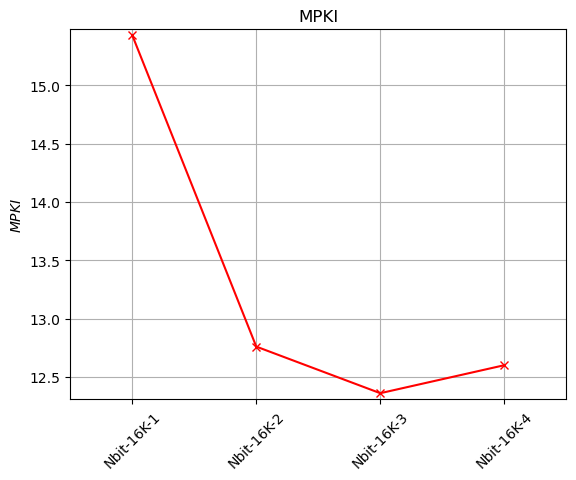
\includegraphics[width=\textwidth]{figures/5_3/401.bzip2.cslab_branch_preds_ref.out.png}
        \caption{401.bzip2}
        \label{fig:plot1}
    \end{subfigure}
    \hfill
    \begin{subfigure}[b]{0.45\textwidth}
        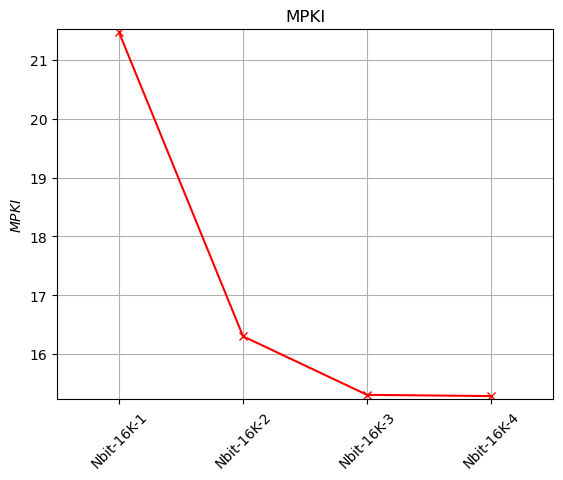
\includegraphics[width=\textwidth]{figures/5_3/403.gcc.cslab_branch_preds_ref.out.png}
        \caption{403.gcc}
        \label{fig:plot2}
    \end{subfigure}

    \vspace{0.5cm} % spacing between rows

    \begin{subfigure}[b]{0.45\textwidth}
        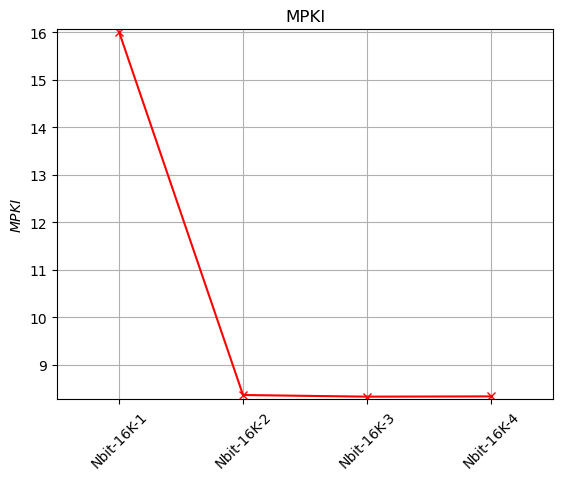
\includegraphics[width=\textwidth]{figures/5_3/410.bwaves.cslab_branch_preds_ref.out.png}
        \caption{410.bwaves}
        \label{fig:plot3}
    \end{subfigure}
    \hfill
    \begin{subfigure}[b]{0.45\textwidth}
        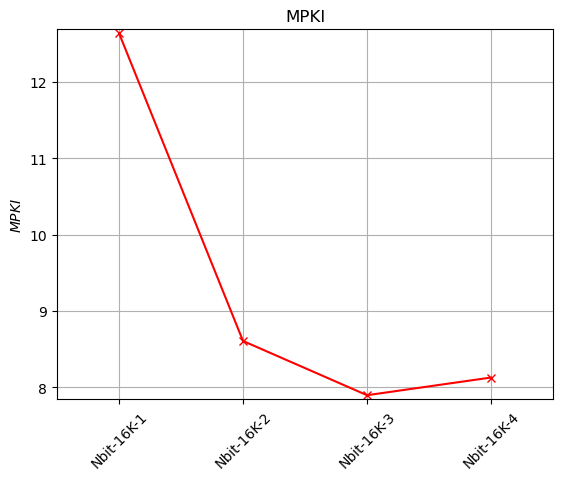
\includegraphics[width=\textwidth]{figures/5_3/416.gamess.cslab_branch_preds_ref.out.png}
        \caption{416.gamess}
        \label{fig:plot4}
    \end{subfigure}

    \vspace{0.5cm} % spacing between rows

    \begin{subfigure}[b]{0.45\textwidth}
        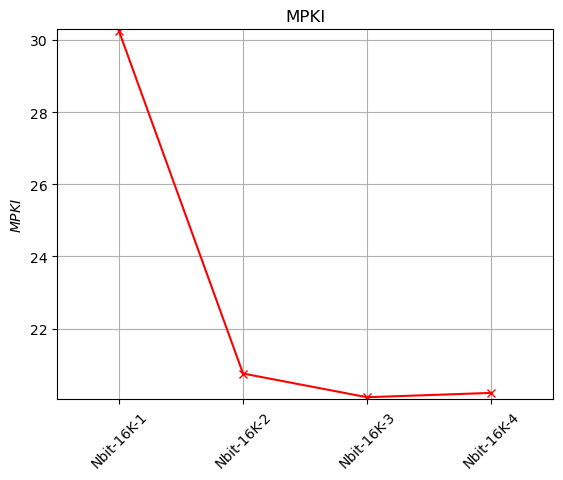
\includegraphics[width=\textwidth]{figures/5_3/429.mcf.cslab_branch_preds_ref.out.png}
        \caption{429.mcf}
        \label{fig:plot5}
    \end{subfigure}
    \hfill
    \begin{subfigure}[b]{0.45\textwidth}
        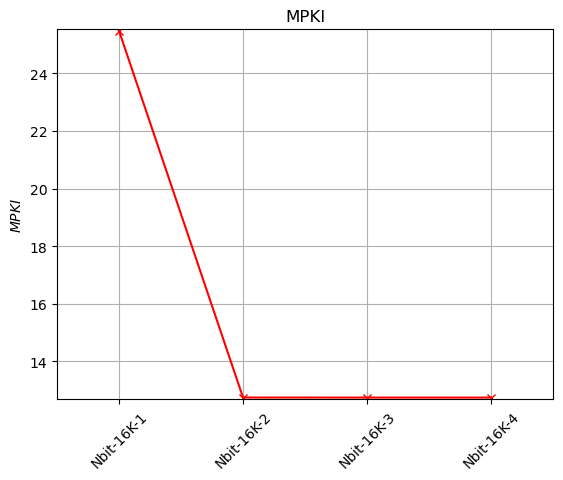
\includegraphics[width=\textwidth]{figures/5_3/433.milc.cslab_branch_preds_ref.out.png}
        \caption{433.milc}
        \label{fig:plot6}
    \end{subfigure}
    \vspace{0.5cm} 

    \caption{Branch Prediction Accuracy for Different N-bit Predictors}
    \label{fig:all_plots}
\end{figure}

\begin{figure}[H]
    \ContinuedFloat
    \centering

    \begin{subfigure}[b]{0.45\textwidth}
        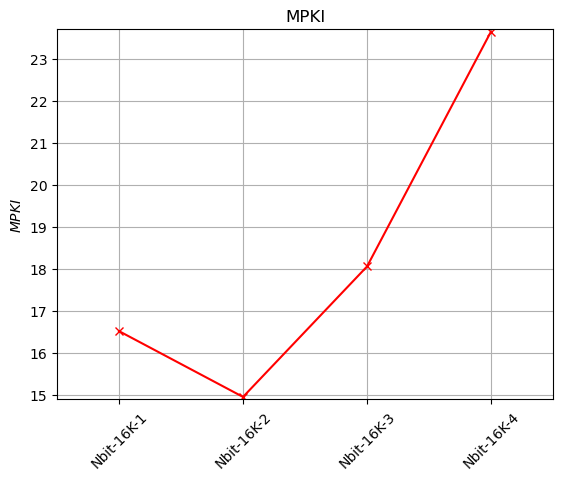
\includegraphics[width=\textwidth]{figures/5_3/435.gromacs.cslab_branch_preds_ref.out.png}
        \caption{435.gromacs}
        \label{fig:plot7}
    \end{subfigure}
    \hfill
    \begin{subfigure}[b]{0.45\textwidth}
        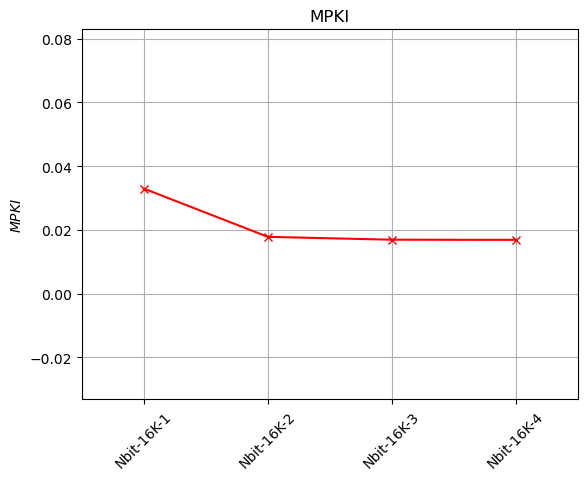
\includegraphics[width=\textwidth]{figures/5_3/436.cactusADM.cslab_branch_preds_ref.out.png}
        \caption{436.cactusADM}
        \label{fig:plot8}
    \end{subfigure}

    \vspace{0.5cm} % spacing between rows

    \begin{subfigure}[b]{0.45\textwidth}
        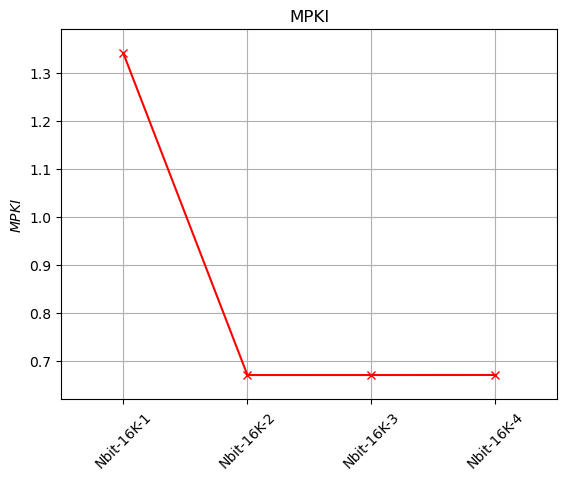
\includegraphics[width=\textwidth]{figures/5_3/437.leslie3d.cslab_branch_preds_ref.out.png}
        \caption{437.leslie3d}
        \label{fig:plot9}
    \end{subfigure}
    \hfill
    \begin{subfigure}[b]{0.45\textwidth}
        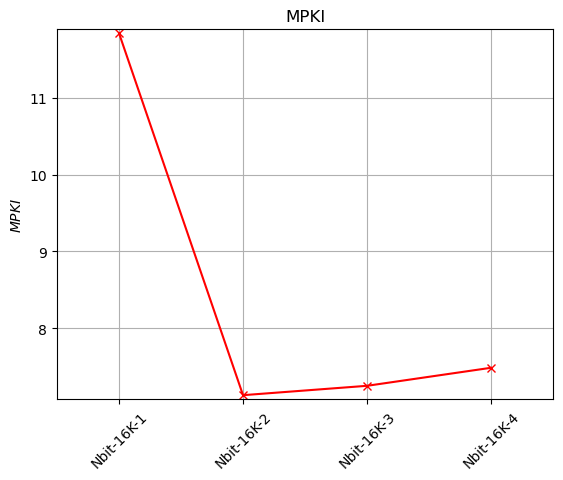
\includegraphics[width=\textwidth]{figures/5_3/450.soplex.cslab_branch_preds_ref.out.png}
        \caption{450.soplex}
        \label{fig:plot10}
    \end{subfigure}

    \vspace{0.5cm} % spacing between rows

    \begin{subfigure}[b]{0.45\textwidth}
        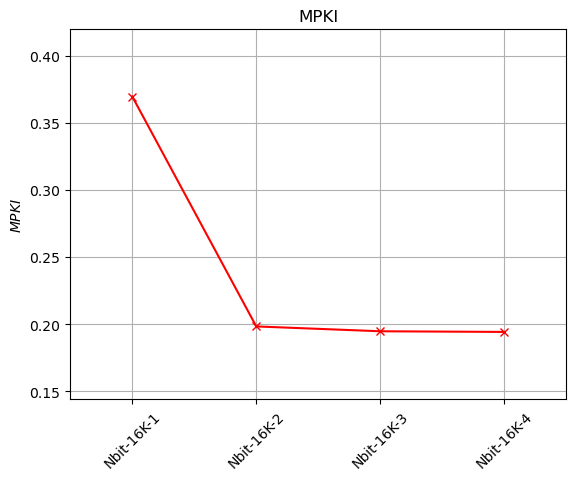
\includegraphics[width=\textwidth]{figures/5_3/456.hmmer.cslab_branch_preds_ref.out.png}
        \caption{456.hmmer}
        \label{fig:plot11}
    \end{subfigure}
    \hfill
    \begin{subfigure}[b]{0.45\textwidth}
        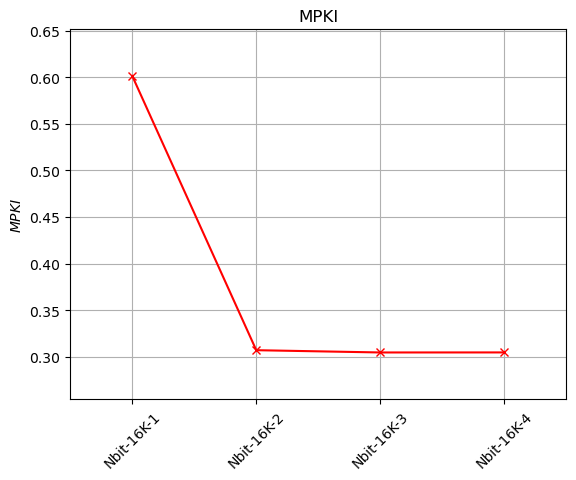
\includegraphics[width=\textwidth]{figures/5_3/459.GemsFDTD.cslab_branch_preds_ref.out.png}
        \caption{459.GemsFDTD}
        \label{fig:plot12}
    \end{subfigure}
    \vspace{0.5cm} 

    \caption{(continued)}
    \label{fig:nbits_part2}
\end{figure}

\begin{figure}[H]
    \ContinuedFloat
    \centering

    \begin{subfigure}[b]{0.45\textwidth}
        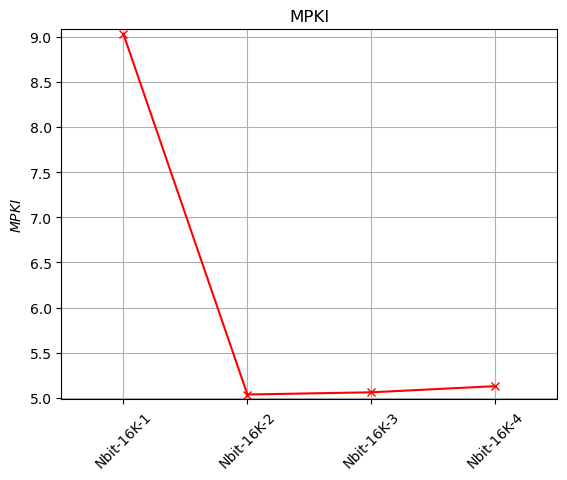
\includegraphics[width=\textwidth]{figures/5_3/464.h264ref.cslab_branch_preds_ref.out.png}
        \caption{464.h264ref}
        \label{fig:plot13}
    \end{subfigure}
    \hfill
    \begin{subfigure}[b]{0.45\textwidth}
        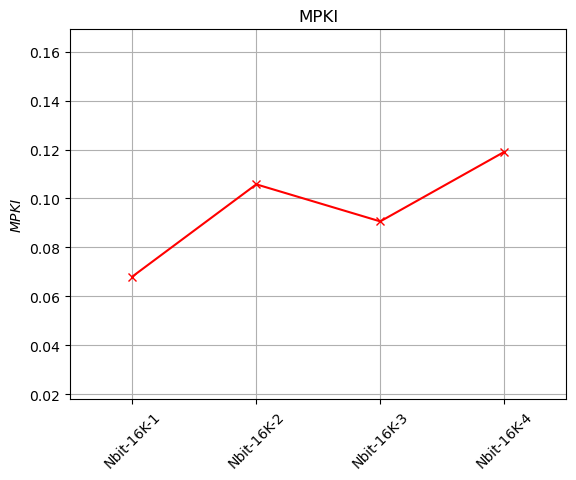
\includegraphics[width=\textwidth]{figures/5_3/470.lbm.cslab_branch_preds_ref.out.png}
        \caption{470.lbm}
        \label{fig:plot14}
    \end{subfigure}

    \vspace{0.5cm} % spacing between rows

    \begin{subfigure}[b]{0.45\textwidth}
        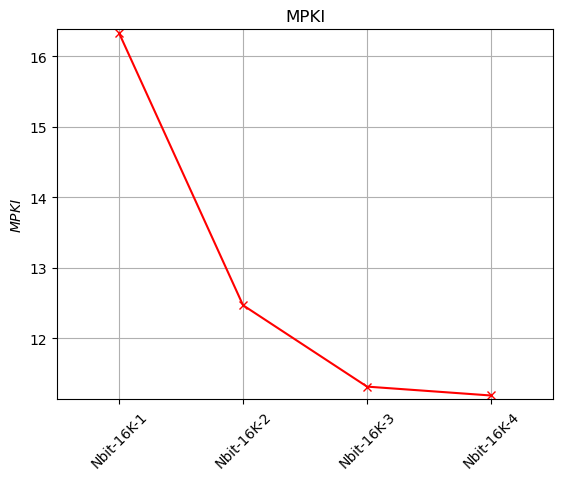
\includegraphics[width=\textwidth]{figures/5_3/471.omnetpp.cslab_branch_preds_ref.out.png}
        \caption{471.omnetpp}
        \label{fig:plot15}
    \end{subfigure}
    \hfill
    \begin{subfigure}[b]{0.45\textwidth}
        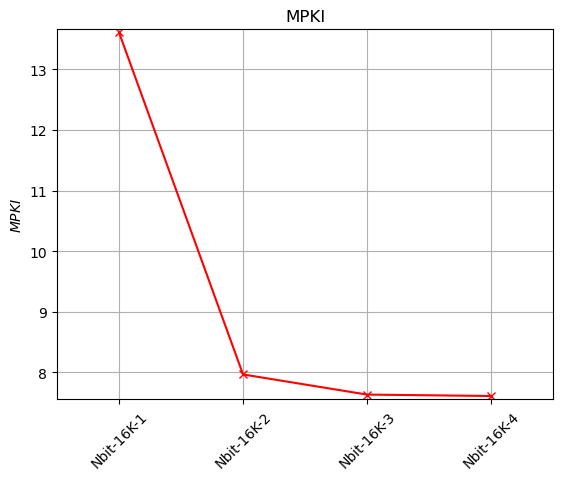
\includegraphics[width=\textwidth]{figures/5_3/483.xalancbmk.cslab_branch_preds_ref.out.png}
        \caption{483.xalancbmk}
        \label{fig:plot16}
    \end{subfigure}

    \vspace{0.5cm} 

    \caption{(continued)}
    \label{fig:nbits_part3}
\end{figure}

Υπολογίζουμε τον γεωμετρικό μέσο όρο του MPKI για κάθε benchmark και για κάθε n-bit predictor. 




\end{document}
